% ==============================================================================
% Chapter 3: System Design
% ==============================================================================
\chapter{System Design}
\label{chap:system_design}

\section{Design Approach}
\label{sec:design_approach}

System design constitutes the foundational architectural bridge transforming the functional requirements, performance specifications, and domain constraints established in Chapter~\ref{chap:requirements} into a concrete, maintainable, and scalable software implementation. For the PocketLaw platform, the software architecture is formulated upon an \textbf{Object-Oriented Design (OOD) Paradigm} coupled with a \textbf{Layered Decoupled Micro-service Architecture}.

The object-oriented paradigm was selected because legal entities, statutory constructs, and transactional interactions possess natural domain boundaries, state encapsulations, and hierarchical relationships:
\begin{itemize}
    \item \textbf{Encapsulation of Relational State:} Core domain concepts---such as Users, Consultations, Chat Messages, Precedent Bookmarks, and Legal Instruments---are encapsulated as discrete SQLAlchemy Declarative Base classes (`User`, `ChatSession`, `ChatMessage`, `SavedDocument`, `CaseBookmark`). Each class encapsulates its internal column schema, foreign key constraints, relationship accessors, and serialization methods (`to_dict()`), preventing uncontrolled mutation across application layers.
    \item \textbf{Polymorphism in Document Compilation:} The document generation engine (`document_generator.py`) applies polymorphic design patterns where the abstract document compilation pipeline coordinates distinct concrete formatting handlers (`format_fir_text`, `format_notice_text`, `format_affidavit_text`, `format_complaint_text`). Each handler encapsulates the idiosyncratic statutory clauses, jurisdictional averments, and notarization jurats required for that specific instrument while adhering to a unified interface returning both formatted text and binary PDF streams.
    \item \textbf{Separation of Concerns across Architectural Tiers:} The system enforces a strict four-layer operational separation:
    \begin{enumerate}
        \item \textit{Presentation Layer:} Client-side reactive UI components and view controllers (React 18 SPA).
        \item \textit{Application \& Security Gateway Layer:} RESTful HTTP routing, JWT token verification, and payload validation (Flask).
        \item \textit{Domain Intelligence Layer:} High-dimensional vector projection, cosine similarity search, and hybrid synthesis (`app.py`, `gemini_service.py`).
        \item \textit{Persistence \& Typography Layer:} ACID relational storage (SQLite 3 WAL) and vector graphics compilation (ReportLab).
    \end{enumerate}
\end{itemize}

\section{Detail Design}
\label{sec:detail_design}

This section delivers an exhaustive structural and behavioural design of PocketLaw utilizing standardized structured analysis tools, Data Flow Diagrams (DFDs), Unified Modelling Language (UML) diagrams, and Entity-Relationship database schemas. All diagrams are rendered on a clean, light/white background strictly complying with GNDEC specifications.

\subsection{System Architecture and Block Diagram}
Figure~\ref{fig:detailed_system_architecture} illustrates the end-to-end component decomposition of the PocketLaw platform, mapping client interactions through the security gateway, algorithmic intelligence core, and persistence engines.

\begin{figure}[H]
\centering
\begin{tikzpicture}[
    node distance=1.1cm and 1.2cm,
    proc/.style={rectangle, draw=blue!80!black, fill=white, thick, rounded corners=3pt, text width=3.8cm, align=center, minimum height=1.0cm, font=\footnotesize},
    store/.style={cylinder, draw=purple!80!black, fill=white, thick, shape border rotate=90, aspect=0.25, text width=3.2cm, align=center, minimum height=1.0cm, font=\footnotesize},
    ext/.style={rectangle, draw=orange!80!black, fill=white, thick, dashed, text width=3.4cm, align=center, minimum height=1.0cm, font=\footnotesize},
    flow/.style={thick, ->, >=stealth, draw=blue!70!black}
]
    % Client Layer
    \node[proc] (react) {\textbf{React 18 Client SPA}\\React Router v6, Axios, Lucide Icons, Chart.js};
    
    % API Gateway
    \node[proc, below=1.0cm of react] (gateway) {\textbf{Flask API Gateway}\\Port 5001, CORS, JWT Auth, Request Dispatcher};
    
    % Intelligence Core
    \node[proc, below left=1.2cm and 0.4cm of gateway] (tfidf) {\textbf{TF-IDF Vector Engine}\\15,000 N-Gram Vocab, Cosine Similarity ($\tau=0.05$)};
    \node[proc, below right=1.2cm and 0.4cm of gateway] (gen) {\textbf{Hybrid Synthesis Engine}\\Prompt Grounding Guard / Local Extractive Synthesizer};
    
    % Persistence and External
    \node[store, below=1.3cm of tfidf] (db) {\textbf{SQLite 3 Relational DB}\\WAL Mode, SQLAlchemy, 5 Normalized Tables};
    \node[proc, below=1.3cm of gen] (reportlab) {\textbf{ReportLab PDF Engine}\\Vector Typography, Court Formats, Notary Jurats};
    \node[ext, right=0.8cm of gen] (gemini) {\textbf{Google Gemini API}\\Multi-Model Failover (Flash-Lite / 3.8-Flash)};
    \node[store, left=0.8cm of tfidf] (scdb) {\textbf{Supreme Court KB}\\2,290 Chunks, 148 Landmark Decisions};

    % Connections
    \draw[flow] (react) -- node[right, font=\tiny] {REST / JSON} (gateway);
    \draw[flow] (gateway) -| (tfidf);
    \draw[flow] (gateway) -| (gen);
    \draw[flow] (scdb) -- node[above, font=\tiny] {Index} (tfidf);
    \draw[flow] (tfidf) -- node[above, font=\tiny] {Ranked Chunks} (gen);
    \draw[flow, <->] (gen) -- node[above, font=\tiny] {API Call} (gemini);
    \draw[flow] (gateway) |- (db);
    \draw[flow] (gateway) |- (reportlab);
    \draw[flow] (reportlab) -- ++(0,-1.0) -| (react);
\end{tikzpicture}
\caption{Detailed Component-Level System Architecture of PocketLaw}
\label{fig:detailed_system_architecture}
\end{figure}

\subsection{Data Flow Diagrams (DFDs)}

Data Flow Diagrams graphically model the information pipeline, depicting how unstructured citizen grievances are transformed into structured legal evaluations, ranked judicial precedents, and court-admissible instruments.

\subsubsection{DFD Level 0 (Context-Level Diagram)}
The context-level DFD captures the macroscopic boundary of the system, illustrating external entities interacting with the primary PocketLaw process.

\begin{figure}[H]
\centering
\begin{tikzpicture}[
    node distance=2.2cm,
    entity/.style={rectangle, draw=black, fill=white, thick, minimum width=3.0cm, minimum height=1.2cm, align=center, font=\small\bfseries},
    process/.style={circle, draw=blue!80!black, fill=white, thick, minimum size=3.2cm, align=center, font=\small\bfseries},
    flow/.style={thick, ->, >=stealth, draw=blue!70!black}
]
    \node[process] (sys) {PocketLaw\\System\\(Process 0.0)};
    \node[entity, left=2.8cm of sys] (user) {Aggrieved Citizen /\\Litigant};
    \node[entity, right=2.8cm of sys] (court) {Police / District Court /\\Consumer Forum};

    \draw[flow] (user.north east) -- node[above, font=\footnotesize, sloped] {Grievance / Form Data} (sys.north west);
    \draw[flow] (sys.south west) -- node[below, font=\footnotesize, sloped] {Legal Advice / Precedents} (user.south east);
    \draw[flow] (sys.east) -- node[above, font=\footnotesize] {Formal Vector PDF Drafts} (court.west);
\end{tikzpicture}
\caption{Data Flow Diagram: Level 0 (Context Diagram)}
\label{fig:dfd_level_0}
\end{figure}

\subsubsection{DFD Level 1 (Functional Decomposition)}
Level 1 DFD decomposes Process 0.0 into its five primary constituent sub-processes: Authentication, Legal Consultation, Precedent Retrieval, Document Generation, and Data Persistence.

\begin{figure}[H]
\centering
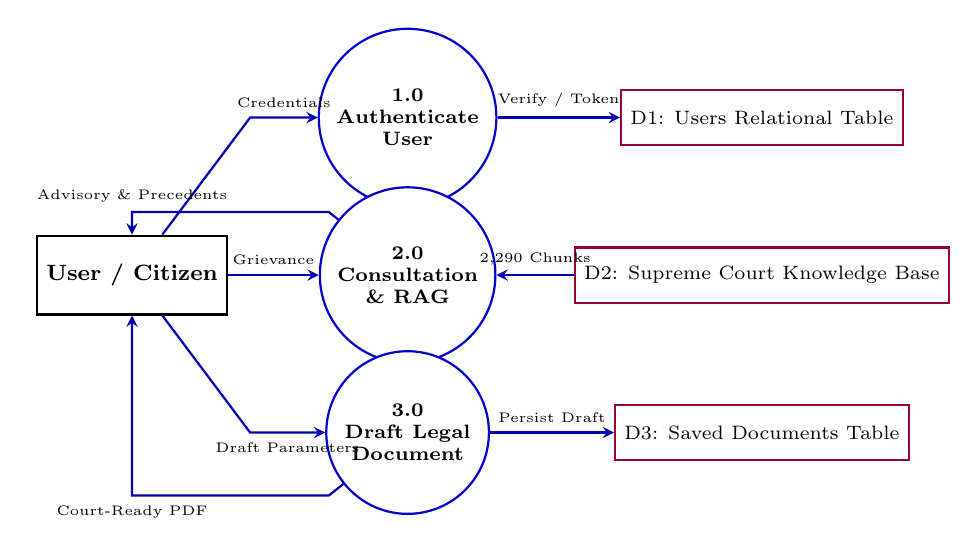
\begin{tikzpicture}[
    node distance=1.4cm and 1.8cm,
    proc/.style={circle, draw=blue!80!black, fill=white, thick, minimum size=2.0cm, align=center, font=\scriptsize\bfseries},
    entity/.style={rectangle, draw=black, fill=white, thick, minimum width=2.4cm, minimum height=1.0cm, align=center, font=\footnotesize\bfseries},
    store/.style={rectangle, draw=purple!80!black, fill=white, thick, minimum width=2.8cm, minimum height=0.7cm, align=center, font=\scriptsize},
    flow/.style={thick, ->, >=stealth, draw=blue!70!black}
]
    \node[entity] (user) at (0, 0) {User / Citizen};
    
    \node[proc] (p1) at (3.5, 2.0) {1.0\\Authenticate\\User};
    \node[proc] (p2) at (3.5, 0.0) {2.0\\Consultation\\\& RAG};
    \node[proc] (p3) at (3.5, -2.0) {3.0\\Draft Legal\\Document};
    
    \node[store] (d1) at (8.0, 2.0) {D1: Users Relational Table};
    \node[store] (d2) at (8.0, 0.0) {D2: Supreme Court Knowledge Base};
    \node[store] (d3) at (8.0, -2.0) {D3: Saved Documents Table};

    \draw[flow] (user) -- ++(1.5, 2.0) -- node[above, font=\tiny] {Credentials} (p1);
    \draw[flow] (user) -- node[above, font=\tiny] {Grievance} (p2);
    \draw[flow] (user) -- ++(1.5, -2.0) -- node[below, font=\tiny] {Draft Parameters} (p3);

    \draw[flow] (p1) -- node[above, font=\tiny] {Verify / Token} (d1);
    \draw[flow] (d2) -- node[above, font=\tiny] {2,290 Chunks} (p2);
    \draw[flow] (p3) -- node[above, font=\tiny] {Persist Draft} (d3);

    \draw[flow] (p2) -- ++(-1.0, 0.8) -| node[above, font=\tiny] {Advisory \& Precedents} (user);
    \draw[flow] (p3) -- ++(-1.0, -0.8) -| node[below, font=\tiny] {Court-Ready PDF} (user);
\end{tikzpicture}
\caption{Data Flow Diagram: Level 1 (Functional Decomposition)}
\label{fig:dfd_level_1}
\end{figure}

\subsubsection{DFD Level 2 (Decomposition of Consultation \& RAG Process 2.0)}
Level 2 DFD drills into Process 2.0 to reveal the internal algorithmic sequence: Normalization, Vector Transformation, Cosine Scoring, Precedent Selection, and Grounded Synthesis.

\begin{figure}[H]
\centering
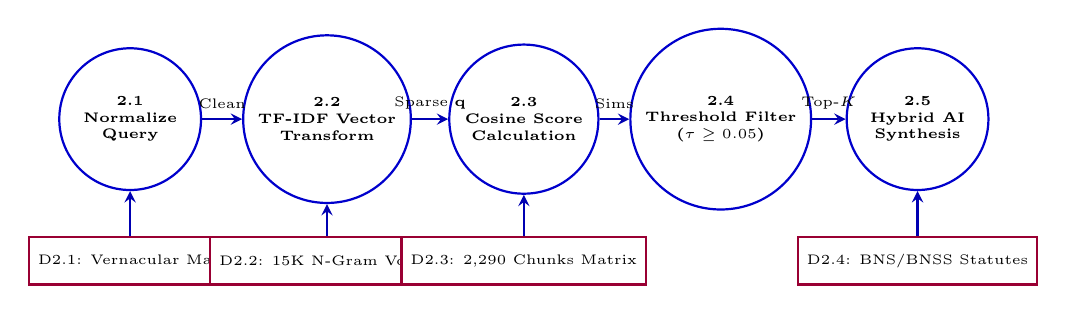
\begin{tikzpicture}[
    node distance=1.1cm,
    proc/.style={circle, draw=blue!80!black, fill=white, thick, minimum size=1.8cm, align=center, font=\tiny\bfseries},
    store/.style={rectangle, draw=purple!80!black, fill=white, thick, minimum width=2.4cm, minimum height=0.6cm, align=center, font=\tiny},
    flow/.style={thick, ->, >=stealth, draw=blue!70!black}
]
    \node[proc] (p21) at (0, 0) {2.1\\Normalize\\Query};
    \node[proc] (p22) at (2.5, 0) {2.2\\TF-IDF Vector\\Transform};
    \node[proc] (p23) at (5.0, 0) {2.3\\Cosine Score\\Calculation};
    \node[proc] (p24) at (7.5, 0) {2.4\\Threshold Filter\\($\tau \ge 0.05$)};
    \node[proc] (p25) at (10.0, 0) {2.5\\Hybrid AI\\Synthesis};

    \node[store] (hmap) at (0, -1.8) {D2.1: Vernacular Map};
    \node[store] (vocab) at (2.5, -1.8) {D2.2: 15K N-Gram Vocab};
    \node[store] (chunks) at (5.0, -1.8) {D2.3: 2,290 Chunks Matrix};
    \node[store] (laws) at (10.0, -1.8) {D2.4: BNS/BNSS Statutes};

    \draw[flow] (p21) -- node[above, font=\tiny] {Clean} (p22);
    \draw[flow] (p22) -- node[above, font=\tiny] {Sparse $\mathbf{q}$} (p23);
    \draw[flow] (p23) -- node[above, font=\tiny] {Sims} (p24);
    \draw[flow] (p24) -- node[above, font=\tiny] {Top-$K$} (p25);

    \draw[flow] (hmap) -- (p21);
    \draw[flow] (vocab) -- (p22);
    \draw[flow] (chunks) -- (p23);
    \draw[flow] (laws) -- (p25);
\end{tikzpicture}
\caption{Data Flow Diagram: Level 2 (Consultation and RAG Sub-processes)}
\label{fig:dfd_level_2}
\end{figure}

\subsection{UML Diagrams}

Unified Modelling Language (UML) diagrams provide formal object-oriented structural and behavioural representations of the system.

\subsubsection{UML Use Case Diagram}
The Use Case Diagram depicts interactions between system actors (Unregistered Citizen, Authenticated Litigant, System Administrator) and core system functionalities.

\begin{figure}[H]
\centering
\begin{tikzpicture}[
    scale=0.88, transform shape,
    actor/.style={circle, draw=black, fill=white, thick, minimum size=0.8cm},
    usecase/.style={ellipse, draw=blue!80!black, fill=white, thick, text width=3.4cm, align=center, minimum height=0.9cm, font=\scriptsize},
    boundary/.style={rectangle, draw=gray!60, fill=white, dashed, inner sep=0.5cm, rounded corners=5pt}
]
    % Actors
    \node[actor] (anon) at (-4.5, 1.5) {};
    \node[below=0.1cm of anon, font=\footnotesize\bfseries] {Unregistered Citizen};
    
    \node[actor] (auth) at (-4.5, -2.5) {};
    \node[below=0.1cm of auth, font=\footnotesize\bfseries] {Registered Litigant};

    % Use Cases
    \node[usecase] (uc1) at (0, 3.0) {Submit Natural Language Grievance};
    \node[usecase] (uc2) at (0, 1.8) {Search Supreme Court Precedents};
    \node[usecase] (uc3) at (0, 0.6) {Browse Modern Statutes (BNS 2023)};
    \node[usecase] (uc4) at (0, -0.6) {Generate Live Document Preview};
    \node[usecase] (uc5) at (0, -1.8) {Download Court-Ready Vector PDF};
    \node[usecase] (uc6) at (0, -3.0) {Bookmark Judgment Precedents};
    \node[usecase] (uc7) at (0, -4.2) {Manage Profile \& Saved Drafts};

    % Associations
    \draw[thick] (anon) -- (uc1);
    \draw[thick] (anon) -- (uc2);
    \draw[thick] (anon) -- (uc3);
    \draw[thick] (anon) -- (uc4);
    \draw[thick] (anon) -- (uc5);

    \draw[thick] (auth) -- (uc1);
    \draw[thick] (auth) -- (uc4);
    \draw[thick] (auth) -- (uc5);
    \draw[thick] (auth) -- (uc6);
    \draw[thick] (auth) -- (uc7);

    % System Boundary
    \begin{scope}[on background layer]
        \node[boundary, fit=(uc1) (uc2) (uc3) (uc4) (uc5) (uc6) (uc7), label=above:{\small\textbf{PocketLaw System Boundary}}] {};
    \end{scope}
\end{tikzpicture}
\caption{UML Use Case Diagram for PocketLaw Platform}
\label{fig:uml_use_case}
\end{figure}

\subsubsection{UML Class Diagram}
The Class Diagram formalizes the relational entities, their internal attributes, data types, and structural multiplicities managed via SQLAlchemy ORM.

\begin{figure}[H]
\centering
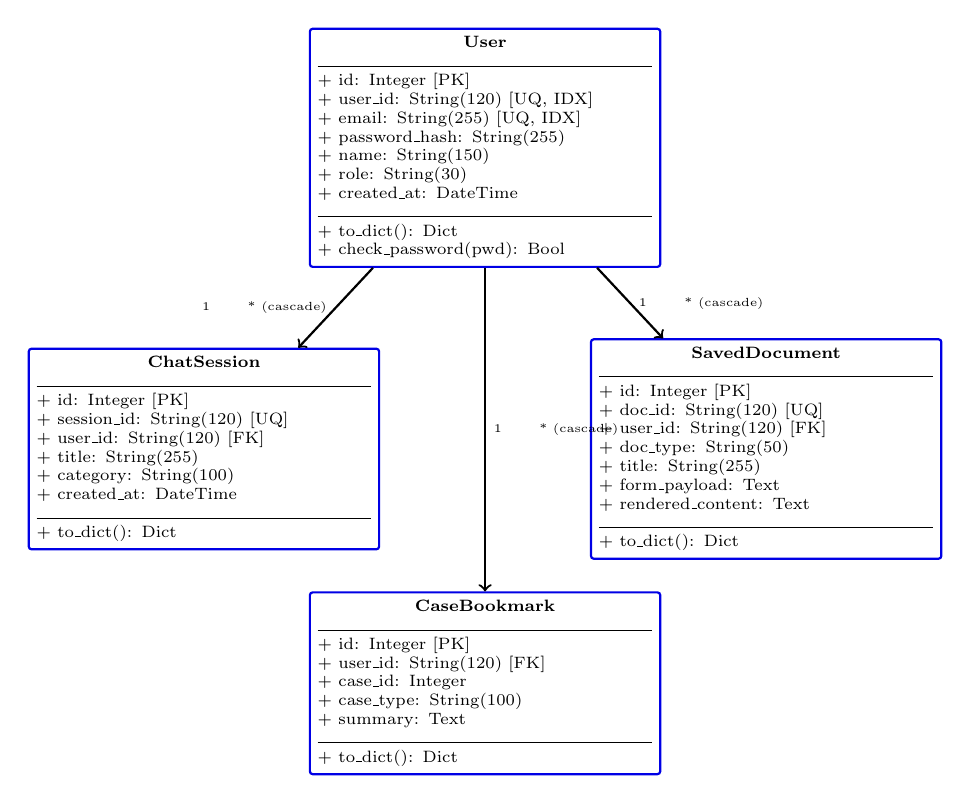
\begin{tikzpicture}[
    scale=0.85, transform shape,
    classbox/.style={rectangle, draw=blue!90!black, fill=white, thick, rounded corners=1pt, text width=5.0cm, font=\scriptsize}
]
    % User Class
    \node[classbox] (user) at (0, 3.5) {
        \textbf{\centerline{User}} \\
        \rule{5.0cm}{0.4pt} \\
        + id: Integer [PK] \\
        + user\_id: String(120) [UQ, IDX] \\
        + email: String(255) [UQ, IDX] \\
        + password\_hash: String(255) \\
        + name: String(150) \\
        + role: String(30) \\
        + created\_at: DateTime \\
        \rule{5.0cm}{0.4pt} \\
        + to\_dict(): Dict \\
        + check\_password(pwd): Bool
    };

    % ChatSession Class
    \node[classbox] (session) at (-4.2, -1.0) {
        \textbf{\centerline{ChatSession}} \\
        \rule{5.0cm}{0.4pt} \\
        + id: Integer [PK] \\
        + session\_id: String(120) [UQ] \\
        + user\_id: String(120) [FK] \\
        + title: String(255) \\
        + category: String(100) \\
        + created\_at: DateTime \\
        \rule{5.0cm}{0.4pt} \\
        + to\_dict(): Dict
    };

    % SavedDocument Class
    \node[classbox] (doc) at (4.2, -1.0) {
        \textbf{\centerline{SavedDocument}} \\
        \rule{5.0cm}{0.4pt} \\
        + id: Integer [PK] \\
        + doc\_id: String(120) [UQ] \\
        + user\_id: String(120) [FK] \\
        + doc\_type: String(50) \\
        + title: String(255) \\
        + form\_payload: Text \\
        + rendered\_content: Text \\
        \rule{5.0cm}{0.4pt} \\
        + to\_dict(): Dict
    };

    % CaseBookmark Class
    \node[classbox] (bm) at (0, -4.5) {
        \textbf{\centerline{CaseBookmark}} \\
        \rule{5.0cm}{0.4pt} \\
        + id: Integer [PK] \\
        + user\_id: String(120) [FK] \\
        + case\_id: Integer \\
        + case\_type: String(100) \\
        + summary: Text \\
        \rule{5.0cm}{0.4pt} \\
        + to\_dict(): Dict
    };

    % Associations
    \draw[thick, ->] (user) -- node[left, font=\tiny] {1 \quad\quad * (cascade)} (session);
    \draw[thick, ->] (user) -- node[right, font=\tiny] {1 \quad\quad * (cascade)} (doc);
    \draw[thick, ->] (user) -- node[right, font=\tiny] {1 \quad\quad * (cascade)} (bm);
\end{tikzpicture}
\caption{UML Class Diagram Depicting Relational Entities and ORM Relationships}
\label{fig:uml_class_diagram}
\end{figure}

\subsubsection{UML Sequence Diagram}
The Sequence Diagram depicts the chronological message interchange between the user interface, API gateway, RAG vector search, hybrid generative synthesis, and persistence layers during a legal consultation.

\begin{figure}[H]
\centering
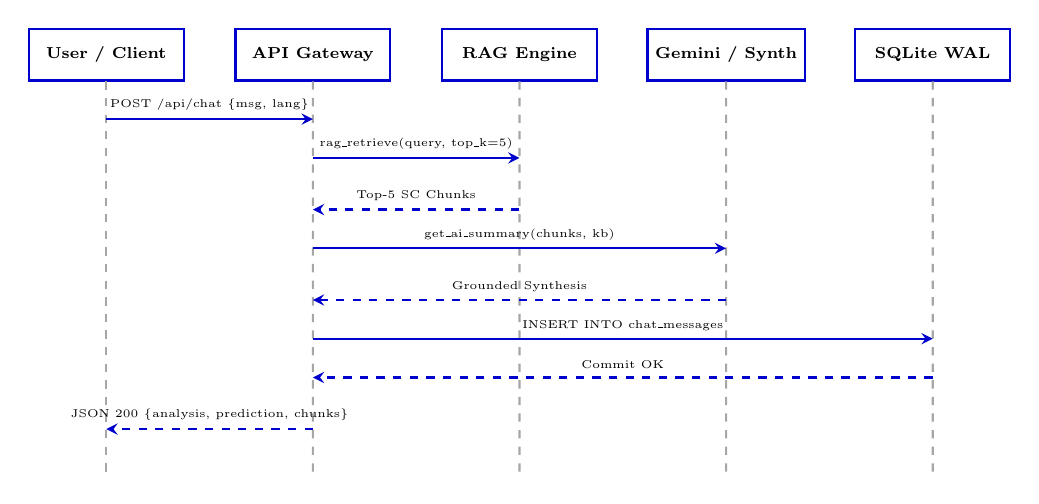
\begin{tikzpicture}[
    scale=0.82, transform shape,
    lifeline/.style={thick, dashed, draw=gray!70},
    obj/.style={rectangle, draw=blue!80!black, fill=white, thick, minimum width=2.4cm, minimum height=0.8cm, align=center, font=\scriptsize\bfseries},
    msg/.style={thick, ->, >=stealth, draw=blue!80!black},
    ret/.style={thick, dashed, ->, >=stealth, draw=blue!80!black}
]
    % Objects
    \node[obj] (c) at (0, 0) {User / Client};
    \node[obj] (g) at (3.2, 0) {API Gateway};
    \node[obj] (r) at (6.4, 0) {RAG Engine};
    \node[obj] (s) at (9.6, 0) {Gemini / Synth};
    \node[obj] (d) at (12.8, 0) {SQLite WAL};

    % Lifelines
    \draw[lifeline] (c) -- (0, -6.5);
    \draw[lifeline] (g) -- (3.2, -6.5);
    \draw[lifeline] (r) -- (6.4, -6.5);
    \draw[lifeline] (s) -- (9.6, -6.5);
    \draw[lifeline] (d) -- (12.8, -6.5);

    % Messages
    \draw[msg] (0, -1.0) -- node[above, font=\tiny] {POST /api/chat \{msg, lang\}} (3.2, -1.0);
    \draw[msg] (3.2, -1.6) -- node[above, font=\tiny] {rag\_retrieve(query, top\_k=5)} (6.4, -1.6);
    \draw[ret] (6.4, -2.4) -- node[above, font=\tiny] {Top-5 SC Chunks} (3.2, -2.4);
    
    \draw[msg] (3.2, -3.0) -- node[above, font=\tiny] {get\_ai\_summary(chunks, kb)} (9.6, -3.0);
    \draw[ret] (9.6, -3.8) -- node[above, font=\tiny] {Grounded Synthesis} (3.2, -3.8);

    \draw[msg] (3.2, -4.4) -- node[above, font=\tiny] {INSERT INTO chat\_messages} (12.8, -4.4);
    \draw[ret] (12.8, -5.0) -- node[above, font=\tiny] {Commit OK} (3.2, -5.0);

    \draw[ret] (3.2, -5.8) -- node[above, font=\tiny] {JSON 200 \{analysis, prediction, chunks\}} (0, -5.8);
\end{tikzpicture}
\caption{UML Sequence Diagram for Legal Consultation and RAG Synthesis}
\label{fig:uml_sequence_diagram}
\end{figure}

\subsubsection{UML Activity Diagram}
Figure~\ref{fig:uml_activity_diagram} details the sequential operational logic of the hybrid synthesis decision flow, highlighting the failover path from Gemini to local extractive synthesis.

\begin{figure}[H]
\centering
\begin{tikzpicture}[
    scale=0.85, transform shape,
    start/.style={circle, draw=black, fill=black, minimum size=0.4cm},
    stop/.style={circle, draw=black, fill=white, line width=1.5pt, minimum size=0.5cm},
    action/.style={rectangle, draw=blue!80!black, fill=white, thick, rounded corners=3pt, text width=3.8cm, align=center, minimum height=0.8cm, font=\scriptsize},
    decision/.style={diamond, draw=orange!90!black, fill=white, thick, aspect=1.8, text width=2.4cm, align=center, font=\tiny},
    arrow/.style={thick, ->, >=stealth, draw=blue!70!black}
]
    \node[start] (s) at (0, 0) {};
    \node[action, below=0.6cm of s] (norm) {Normalize Vernacular Terminology};
    \node[action, below=0.6cm of norm] (rag) {Compute Cosine Similarity on 2,290 Chunks};
    \node[decision, below=0.6cm of rag] (dec1) {GEMINI\_API\_KEY Configured?};
    \node[action, right=1.2cm of dec1] (gem) {Generate Grounded Gemini Response (8s Timeout)};
    \node[decision, below=0.8cm of gem] (dec2) {API Response Valid?};
    \node[action, below=1.8cm of dec1] (local) {Execute Offline Extractive Synthesis from KB};
    \node[action, below=0.8cm of local] (comb) {Synthesize Final Cards \& Legal Sections};
    \node[stop, below=0.6cm of comb] (end) {};

    \draw[arrow] (s) -- (norm);
    \draw[arrow] (norm) -- (rag);
    \draw[arrow] (rag) -- (dec1);
    \draw[arrow] (dec1) -- node[above, font=\tiny] {Yes} (gem);
    \draw[arrow] (dec1) -- node[left, font=\tiny] {No} (local);
    \draw[arrow] (gem) -- (dec2);
    \draw[arrow] (dec2) |- node[above, font=\tiny] {No (Failover)} (local);
    \draw[arrow] (dec2) |- node[right, font=\tiny] {Yes} (comb);
    \draw[arrow] (local) -- (comb);
    \draw[arrow] (comb) -- (end);
\end{tikzpicture}
\caption{UML Activity Diagram for Hybrid Synthesis and Failover Logic}
\label{fig:uml_activity_diagram}
\end{figure}

\subsubsection{UML Deployment Diagram}
Figure~\ref{fig:uml_deployment_diagram} illustrates the physical deployment topology, showcasing how client browser nodes communicate across network boundaries with the Flask backend runtime and local persistence stores.

\begin{figure}[H]
\centering
\begin{tikzpicture}[
    scale=0.85, transform shape,
    nodebox/.style={rectangle, draw=black, fill=white, thick, text width=5.0cm, minimum height=3.5cm, rounded corners=2pt, font=\scriptsize},
    artifact/.style={rectangle, draw=blue!80!black, fill=white, thick, text width=4.2cm, align=center, minimum height=0.7cm, font=\tiny}
]
    % Client Device Node
    \node[nodebox] (client) at (-3.5, 0) {
        \textbf{\centerline{<<Device: Client Machine>>}} \\
        \textbf{\centerline{Modern Web Browser}} \\[0.3cm]
        \centering
        \begin{tikzpicture}
            \node[artifact] {React 18 SPA (Build Artifacts)};
            \node[artifact, yshift=-0.9cm] {Axios Client Interceptors};
            \node[artifact, yshift=-1.8cm] {Web Audio Speech API};
        \end{tikzpicture}
    };

    % Server Node
    \node[nodebox] (server) at (3.5, 0) {
        \textbf{\centerline{<<Device: Application Host>>}} \\
        \textbf{\centerline{Python 3.14 / Flask Runtime}} \\[0.3cm]
        \centering
        \begin{tikzpicture}
            \node[artifact] {Flask REST API Gateway (Port 5001)};
            \node[artifact, yshift=-0.9cm] {Scikit-Learn TF-IDF VSM (In-Memory)};
            \node[artifact, yshift=-1.8cm] {ReportLab Vector PDF Generator};
        \end{tikzpicture}
    };

    % Database File
    \node[rectangle, draw=purple!80!black, fill=white, thick, text width=4.0cm, align=center, below=1.2cm of server] (dbfile) {
        \textbf{<<File System>>} \\
        `data/pocketlaw.db` (SQLite WAL)
    };

    \draw[thick, <->] (client) -- node[above, font=\scriptsize] {HTTP / HTTPS (TCP 3000/5001)} (server);
    \draw[thick, <->] (server) -- node[right, font=\scriptsize] {Direct File I/O (WAL)} (dbfile);
\end{tikzpicture}
\caption{UML Deployment Diagram of the PocketLaw Application Architecture}
\label{fig:uml_deployment_diagram}
\end{figure}

\subsection{Database Design and Relational Schema}
PocketLaw's data architecture is implemented on SQLite 3 with Write-Ahead Logging (`PRAGMA journal_mode=WAL`), connection pooling (`pool_recycle=300`), and cascade deletion foreign keys.

\subsubsection{Entity-Relationship (E-R) Diagram}
Figure~\ref{fig:er_diagram} depicts the Entity-Relationship schema capturing primary keys, foreign key constraints, and cardinalities.

\begin{figure}[H]
\centering
\begin{tikzpicture}[
    scale=0.85, transform shape,
    entity/.style={rectangle, draw=blue!90!black, fill=white, thick, text width=3.2cm, align=center, minimum height=1.0cm, font=\small\bfseries},
    rel/.style={diamond, draw=orange!90!black, fill=white, thick, text width=1.8cm, align=center, font=\tiny},
    attr/.style={ellipse, draw=gray!80, fill=white, thin, font=\tiny, align=center}
]
    \node[entity] (user) at (0, 0) {USER};
    \node[rel, right=2.0cm of user] (r1) {Owns /\\Initiates};
    \node[entity, right=2.0cm of r1] (session) {CHAT\\SESSION};
    
    \node[rel, below=1.5cm of user] (r2) {Creates /\\Saves};
    \node[entity, below=1.5cm of r2] (doc) {SAVED\\DOCUMENT};

    \node[rel, left=2.0cm of user] (r3) {Pins /\\Saves};
    \node[entity, left=2.0cm of r3] (bm) {CASE\\BOOKMARK};

    \node[rel, below=1.5cm of session] (r4) {Contains};
    \node[entity, below=1.5cm of r4] (msg) {CHAT\\MESSAGE};

    \draw[thick] (user) -- node[above, font=\tiny] {1} (r1);
    \draw[thick, ->] (r1) -- node[above, font=\tiny] {N} (session);
    
    \draw[thick] (user) -- node[left, font=\tiny] {1} (r2);
    \draw[thick, ->] (r2) -- node[left, font=\tiny] {N} (doc);

    \draw[thick] (user) -- node[above, font=\tiny] {1} (r3);
    \draw[thick, ->] (r3) -- node[above, font=\tiny] {N} (bm);

    \draw[thick] (session) -- node[left, font=\tiny] {1} (r4);
    \draw[thick, ->] (r4) -- node[left, font=\tiny] {N} (msg);
\end{tikzpicture}
\caption{Entity-Relationship (E-R) Diagram of PocketLaw Database}
\label{fig:er_diagram}
\end{figure}

\subsubsection{Complete Normalized Relational Tables}
The relational database strictly implements Third Normal Form (3NF). Tables~\ref{tab:schema_users} through~\ref{tab:schema_bookmarks} define the complete physical data dictionary extracted directly from `backend/database.py`.

\begin{table}[H]
\caption{Physical Data Dictionary: `users` Relational Table}
\label{tab:schema_users}
\centering
\small
\begin{tabularx}{\textwidth}{lp{2.8cm}p{2.5cm}X}
\toprule
\textbf{Column Name} & \textbf{Data Type} & \textbf{Constraints} & \textbf{Description / Business Logic} \\
\midrule
`id` & Integer & PK, Auto Increment & Internal surrogate primary key integer. \\
`user_id` & String(120) & Unique, Not Null, Index & Public cryptographic UUID string identifying user. \\
`email` & String(255) & Unique, Not Null, Index & User login email address (case-insensitive). \\
`password_hash` & String(255) & Not Null & Salted PBKDF2 SHA-256 cryptographic password hash. \\
`name` & String(150) & Default: `""` & Full display name of the registered user. \\
`avatar_url` & Text & Default: `""` & Optional external or local avatar image URI. \\
`bio` & Text & Default: `""` & User biographical summary or professional title. \\
`role` & String(30) & Default: `"user"` & Access control role (`user` or `admin`). \\
`created_at` & DateTime & Default: `utcnow` & Timestamp of account registration. \\
`updated_at` & DateTime & Default: `utcnow` & Timestamp of last profile update. \\
\bottomrule
\end{tabularx}
\end{table}

\begin{table}[H]
\caption{Physical Data Dictionary: `chat_sessions` Relational Table}
\label{tab:schema_sessions}
\centering
\small
\begin{tabularx}{\textwidth}{lp{2.8cm}p{2.5cm}X}
\toprule
\textbf{Column Name} & \textbf{Data Type} & \textbf{Constraints} & \textbf{Description / Business Logic} \\
\midrule
`id` & Integer & PK, Auto Increment & Surrogate primary key integer. \\
`session_id` & String(120) & Unique, Not Null, Index & Unique consultation session identifier string. \\
`user_id` & String(120) & FK (`users.user_id`), Index & Owning user reference with `ON DELETE CASCADE`. \\
`title` & String(255) & Default: `"New Consultation"` & Descriptive topic title of the legal session. \\
`category` & String(100) & Default: `"general"` & Detected legal domain (e.g., criminal, consumer). \\
`created_at` & DateTime & Default: `utcnow` & Session creation timestamp. \\
`updated_at` & DateTime & Default: `utcnow` & Last message activity timestamp. \\
\bottomrule
\end{tabularx}
\end{table}

\begin{table}[H]
\caption{Physical Data Dictionary: `chat_messages` Relational Table}
\label{tab:schema_messages}
\centering
\small
\begin{tabularx}{\textwidth}{lp{2.8cm}p{2.5cm}X}
\toprule
\textbf{Column Name} & \textbf{Data Type} & \textbf{Constraints} & \textbf{Description / Business Logic} \\
\midrule
`id` & Integer & PK, Auto Increment & Surrogate primary key integer. \\
`session_id` & String(120) & FK (`chat_sessions`), Index & Parent session reference (`ON DELETE CASCADE`). \\
`user_id` & String(120) & FK (`users.user_id`), Index & Author user reference (`ON DELETE CASCADE`). \\
`role` & String(20) & Default: `"user"` & Message originator (`user` or `assistant`). \\
`message` & Text & Not Null & Raw textual content of grievance or response. \\
`response_preview`& Text & Default: `""` & Truncated preview text for history rendering. \\
`category` & String(100) & Default: `"general"` & Matched substantive statutory classification. \\
`mode` & String(50) & Default: `"both"` & Consultation mode (`rag`, `web`, or `both`). \\
`meta_json` & Text & Default: `"{}"` & Serialized JSON payload containing matched laws. \\
`timestamp` & DateTime & Default: `utcnow`, Index & Exact message arrival timestamp. \\
\bottomrule
\end{tabularx}
\end{table}

\begin{table}[H]
\caption{Physical Data Dictionary: `saved_documents` Relational Table}
\label{tab:schema_documents}
\centering
\small
\begin{tabularx}{\textwidth}{lp{2.8cm}p{2.5cm}X}
\toprule
\textbf{Column Name} & \textbf{Data Type} & \textbf{Constraints} & \textbf{Description / Business Logic} \\
\midrule
`id` & Integer & PK, Auto Increment & Surrogate primary key integer. \\
`doc_id` & String(120) & Unique, Not Null, Index & Public document tracking identifier. \\
`user_id` & String(120) & FK (`users.user_id`), Index & Drafter user reference (`ON DELETE CASCADE`). \\
`doc_type` & String(50) & Not Null, Index & Legal type (`fir`, `notice`, `affidavit`, `complaint`). \\
`title` & String(255) & Not Null & Human-readable document title. \\
`form_payload` & Text & Default: `"{}"` & Serialized JSON dictionary of form field inputs. \\
`rendered_content`& Text & Not Null & Formatted court-ready plain text of the draft. \\
`created_at` & DateTime & Default: `utcnow`, Index & Initial draft generation timestamp. \\
`updated_at` & DateTime & Default: `utcnow` & Last modification timestamp. \\
\bottomrule
\end{tabularx}
\end{table}

\begin{table}[H]
\caption{Physical Data Dictionary: `case_bookmarks` Relational Table}
\label{tab:schema_bookmarks}
\centering
\small
\begin{tabularx}{\textwidth}{lp{2.8cm}p{2.5cm}X}
\toprule
\textbf{Column Name} & \textbf{Data Type} & \textbf{Constraints} & \textbf{Description / Business Logic} \\
\midrule
`id` & Integer & PK, Auto Increment & Surrogate primary key integer. \\
`user_id` & String(120) & FK (`users.user_id`), Index & User reference (`ON DELETE CASCADE`). \\
`case_id` & Integer & Not Null, Index & Supreme Court landmark case identifier. \\
`case_type` & String(100) & Default: `""` & Jurisprudential classification (e.g., Criminal). \\
`year` & String(20) & Default: `""` & Decision year of the judgment. \\
`summary` & Text & Default: `""` & Ground-truth precedent summary. \\
`notes` & Text & Default: `""` & User personal research annotations. \\
`created_at` & DateTime & Default: `utcnow` & Pinned bookmark timestamp. \\
\bottomrule
\end{tabularx}
\end{table}

\section{User Interface Design}
\label{sec:ui_design}

PocketLaw's presentation layer is designed as an accessible, responsive Single Page Application (SPA) adhering to modern UX design principles. Table~\ref{tab:ui_screens} enumerates the layout hierarchy, interaction patterns, and visual components implemented across the ten distinct client-side routes.

\begin{table}[H]
\caption{User Interface Layout and Screen Specification}
\label{tab:ui_screens}
\centering
\small
\begin{tabularx}{\textwidth}{lp{3.2cm}X}
\toprule
\textbf{Route Path} & \textbf{Component Name} & \textbf{Screen Layout, Visual Elements, and Interactive Modalities} \\
\midrule
`/` & `HomePage.jsx` & Hero banner with natural language grievance textarea, language selector (EN, HI, PA, UR), speech recognition mic, prediction metrics (duration, risk level, success rate), and 4 categorized result cards (Laws, Rights, Action Steps, Helplines). \\
\midrule
`/dashboard` & `DashboardPage.jsx` & Analytics dashboard displaying Chart.js case-type distributions, outcome ratios (Allowed vs Dismissed), timeline of judgments, and quick-action shortcuts. \\
\midrule
`/documents` & `DocumentsPage.jsx` & Dual-pane split-screen interface: Left pane houses dynamic tabbed drafting forms (FIR, Notice, Affidavit, Complaint); Right pane renders real-time keystroke live preview with one-click Vector PDF download. \\
\midrule
`/laws` & `LawsPage.jsx` & Interactive statute catalog featuring modern criminal codes (BNS 2023, BNSS 2023, BSA 2023, IT Act, CPA 2019) with colonial IPC/CrPC cross-mapping tables. \\
\midrule
`/search` & `SearchPage.jsx` & Precedent search engine with parametric filters for judgment category, decision year, outcome, and keyword text search with bookmarking toggles. \\
\midrule
`/rag` & `RAGSearchPage.jsx` & Deep semantic vector search interface directly querying the 2,290 Supreme Court chunk matrix, displaying chunk text, cosine similarity score, and source citations. \\
\midrule
`/steps` & `StepsPage.jsx` & Step-by-step procedural playbooks for filing Zero FIRs, consumer grievances on E-Daakhil, cyber fraud reporting on 1930, and bail applications. \\
\midrule
`/history` & `ChatHistoryPage.jsx` & Multi-session consultation archive listing past legal consultations with date filters, message logs, and exportable PDF summaries. \\
\midrule
`/login` & `LoginPage.jsx` & Card-based authentication form with email and password fields, JWT session establishment, and error toast notifications. \\
\midrule
`/profile` & `ProfilePage.jsx` & Litigant profile manager allowing display name edits, password updates, biographical details, and saved document draft archives. \\
\bottomrule
\end{tabularx}
\end{table}

\section{Methodology}
\label{sec:methodology}

The end-to-end operational methodology of PocketLaw follows a rigorous, multi-stage pipeline:
\begin{enumerate}
    \item \textbf{Grievance Normalization and Query Expansion:}
    The incoming natural language query $q$ is converted to lowercase and processed through an Indian vernacular dictionary (`HINDI_MAP`). Terms such as \textit{``chori''} (theft), \textit{``gadi''} (vehicle), \textit{``paise''} (money), and \textit{``talaq''} (divorce) are expanded with canonical legal keywords to optimize token overlap in the vector space.
    
    \item \textbf{High-Dimensional Sparse Vector Projection:}
    The expanded query $q_{exp}$ is projected into the 15,000-dimensional sparse feature space using sublinear Term Frequency-Inverse Document Frequency scaling:
    \begin{equation}
        TF(t, q_{exp}) = 1 + \log(f_{t, q_{exp}}) \quad \text{for } f_{t, q_{exp}} > 0
    \end{equation}
    yielding a unit-normalized sparse vector $\mathbf{q} \in \mathbb{R}^{15000}$.
    
    \item \textbf{Cosine Kernel Precedent Evaluation:}
    The sparse vector $\mathbf{q}$ is multiplied against the pre-compiled Compressed Sparse Row (CSR) matrix $\mathbf{M} \in \mathbb{R}^{2290 \times 15000}$ representing the 2,290 Supreme Court chunks:
    \begin{equation}
        \mathbf{s} = \mathbf{M} \cdot \mathbf{q}^T = \left[ \cos(\mathbf{q}, \mathbf{d}_1), \cos(\mathbf{q}, \mathbf{d}_2), \dots, \cos(\mathbf{q}, \mathbf{d}_{2290}) \right]^T
    \end{equation}
    Candidates satisfying $s_i \ge 0.05$ are sorted in descending order, and the top-$K$ chunks are selected.
    
    \item \textbf{Contextual Fusion and Grounded Synthesis:}
    The retrieved precedent text is combined with structured statutory knowledge from `LAWS_DB`. The hybrid synthesis engine constructs a grounded prompt submitted to Google Gemini or activates the deterministic extractive summarizer, guaranteeing that legal advice remains strictly rooted in verified judicial and legislative text.
    
    \item \textbf{Court-Ready Typography Compilation:}
    When the user initiates document generation, form parameters are serialized and dispatched to the ReportLab engine. The engine compiles an official vector PDF complete with jurisdictional headers, statutory section averments, chronological fact schedules, and formal two-column Notary Jurat attestations.
\end{enumerate}
